%!TEX root = ../main.tex
\chapter{Methodology}\label{chapter:methodology}
In this chapter we outlay how we planned and performed our research.
We will look upon the overall procedure and also discuss on why we chose certain approach.
Let us start with the overview of our experiment.
\section{Overview}
\label{sec:Overview}
Figure~\ref{fig:bigpicture} shows the overall structure of the procedure we followed to perform our research.
We started with old database which had all the analysis result saved for the samples submitted to Anubis.
We made a reverse index from the database such that every resource name had the malware id associated with the resource through some resource activity.
Initially, we took into account resource type \emph{File, Registry, and Mutex}, and the resource activity \emph{create, read, modify, and delete}.\\
After the reverse index was created, we mapped the create activity with read, modify, and delete activities.
As the result of the mapping we had list of malware that created a \textit{resource name}, and a list of malware that either read/modify/delete the same resource name.
We used some heuristics such as resource name created by exactly one single malware and delete by another single malware, to get the candidate pair and run the candidate pair in Anubis system.
We analyzed the result and found some interesting case of dropper malware, self reading malware, and most importantly a logical flaw in our current approach.\\
The flaw in our current approach was we did not had failed attempt of malware activity such as read and delete logged in our database.
This was because every sample binary submitted to anubis system for analysis were run in complete isolation.
Hence any other malware binary which would try to access the resource created by malware other than itself would result into failed access or delete.
We needed this failed operation we needed to create the new database. We used behavioral profile described in~\ref{sec:Behavioral Profile}to recreate the database.\\
We also used document clustering algorithm, discussed in~\autoref{sec:Topic model} to cluster the malware based on their dynamic behavioral activities into different topic families.
We used approach as discussed in~\autoref{sec:Running Experiment} to find the probable candidate pairs.
After we had minimal number of candidate pairs covering all the family topic and interesting resources, we run those pairs in the Anubis system and analyzed the result to find battle activities between the two candidates.
\begin{figure}[htbp]
  \centering
  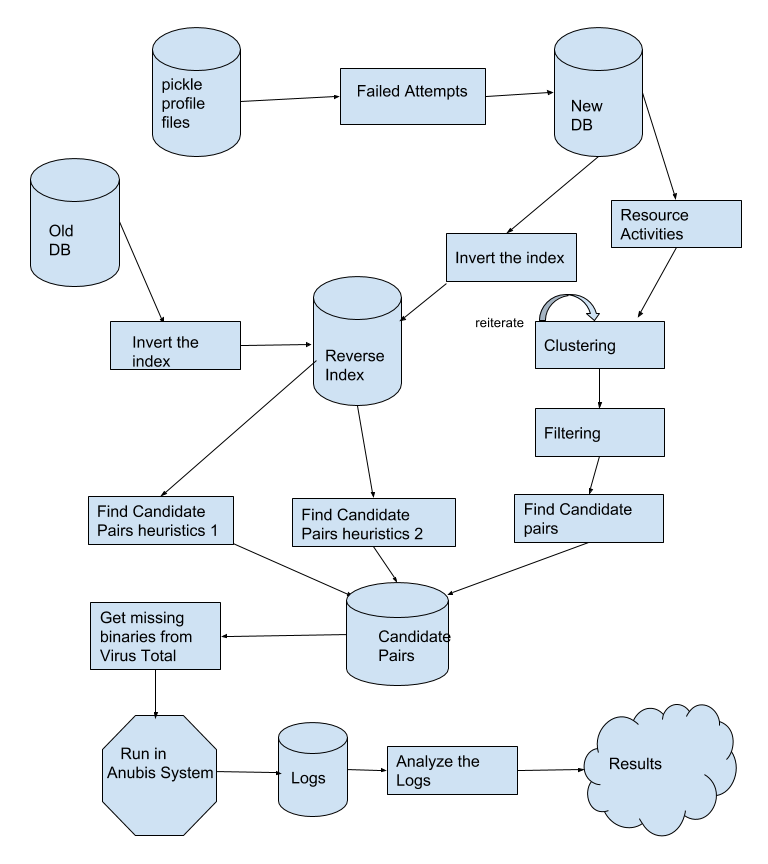
\includegraphics[scale=0.4]{figures/bigpicture.png}
  \caption[Big Picture]{Overview of the research and experiment}\label{fig:bigpicture}
\end{figure}
\section{Behavioral Profile}
\label{sec:Behavioral Profile}
Previously,~\citeauthor{bayer} used Anubis system for the dynamic analysis of malware to gets it execution traces~\cite[]{bayer}.
According to the authors,~\citeauthor{bayer}, ``\textbf{behavioral profile}'', is defined as the abstraction of a program's execution trace that provides information on the OS objects that the program operated on, along with the operations.
As OS Object refers to resource type such as file, registry or section, that could be modified or queried with the system calls.
System calls consisted of Windows NT, native API and the Windows API functions.\\
They created a behavioral profile based on the execution traces of programs irrespective of order execution.
It consisted of a list of different operations operated on the different OS objects during the execution of binary.
The system calls that had same purpose as resultant output but different calling API name were generalized under single name.
We had these behavioral profiles saved as python pickle~\cite[]{pythonpickle} file in our system and we used this to recreate new database that had the record of failed attempts of delete or read.
\\
Our primarily concern was list of \emph{OS Objects} and \emph{Operations} associated with the behavioral profile of the malware.
We needed those to recreate the database with the system calls as malware activities 
Lets describe these two in a brief.
\subsection{OS Objects}
\label{sub:OS Objects}
OS Object were primarily the resource that were created, delete, modified during the program execution.
\citeauthor{bayer} define \emph{OS Objects} as:
\begin{lstlisting}
OS Object ::= (type, object-name)
type ::= file|registry|process|job|
       network|thread|section|
       driver|sync|service|random|
       time|info
\end{lstlisting}
\subsection{OS Operations}
\label{sub:OS Operations}
Broadly, OS Operation is the generalization of a system call.
\citeauthor{bayer} define \emph{OS Operations} as:
\begin{lstlisting}
OS operation ::= (operation-name,
                opeartion-attributes?,
                successful?)
\end{lstlisting}
The sample of behavioral profile is shown in~\autoref{lst:bpsample} in~\autoref{chapter:implementation} where we also describe how we used it for generating resource activities and text corpora for clustering.
\section{Resource Types}
\label{sec:Resource Types}
As discussed before in~\autoref{sub:OS Objects}, an OS Object, are representation of resource types.
For our research, we took into consideration following 8 resource types among those list.
We will give a short description of each resource type according to Microsoft Developers Network documentation.
All the definition are taken into account from Microsoft Developers Network Official documentation website.\cite[MSDN]{msdn}.
\subsection{File}
\label{sub:File}
A \emph{file} is a means of storing resourceful information which can be retrieved or modified in future.
File objects function as the logical interface between kernel and user-mode processes and the file data that resides on the physical disk.
It not only holds the data written on the file but also a set of attributes maintained by the kernel for system purposes such as \emph{File name, Current byte offset, Share mode, I/O mode}~\cite[]{msfile}.\\
File type in the behavioral profile encompasses not only general file, but named pipe and mailslot resources. File is an important resource type for us to focus as our hypothesis for research is that malware of certain family creates or deletes a certain file to infect a system and this also could be used by malware of another family to remove its nemesis from system.
\subsection{Registry}
\label{sub:Registry}
\emph{Registry} is a database defined by a system where different applications and system components store and retrieve data such as configurations settings for its use.
The data stored in the registry varies according to the version of Microsoft Windows.
Application performs the basic add, modify, retrieve, or delete operation in the registry through the registry API~\cite[]{msregistry}.\\
We take the registry keys associated with the malware into consideration for experiment as it provides vital information on the behavior of a malware sample. Malware with same family might have similar registry key activity and also malware from different family might look for the particular registry key in the system in order to detect the presence of its anti family.
\subsection{Service}
\label{sub:Service}
A user can start a \emph{service} automatically at system boot through the Service Control Panel, or an application can also use service functions such as \emph{StartService, OpenService, DeleteService} to configure services.
However, it must conform to the interface rules of Service Control Manater (SCM)~\cite[]{msservice}.
\subsection{Section}
\label{sub:Section}
A \emph{section} object is sharable memory which is used by process to share its memory address space (memory sections) with other processes.
It is also used by process to map a file into its memory address space~\cite[]{mssection}.\\
In case of behavioral profile, it broadly represents memory mapped files.
\subsection{Process}
\label{sub:Process}
A binary can spawn one or more \emph{processes}
A process is simply an instance of a computer program being executed that consists of instructions and current activity of program.
One or more threads can be run in the context of the process~\cite[]{msprocess} 
\subsection{Job}
\label{sub:Job}
\emph{Job} object makes grouping of process as single unit  to manage possible.
It can be named and shared securely to control attributes of processes grouped together and operation on a job makes the affect on all the process in its group~\cite[]{msjob}.
\subsection{Sync}
\label{sub:Sync}
A \emph{sync object} is used to coordinate the execution of multiple threads as more than one process could share the handle of single synchronization object which helps for the interprocess synchronization between these processes~\cite[]{mssync}.\\
The sync object type covers all the synchronization activities.
\cite[]{mssync}.
\subsection{Driver}
\label{sub:Driver}
A \emph{device driver } is a program that is associated with certain device for its operation and control. It is used as an software interface to communicate between the hardware device and the operating system and other software~\cite[Device Driver]{devicedriver} \\
Windows represent devices with device objects, and one device could be represented by more than one device objects. All operation on device is conducted via device object~\cite[]{msdevice}.\\
We capture those loading and unloading of Windows Device Driver recorded in the behavioral profile.
% \section{Topic modeling}
% \label{sec:Topic model}
% We started to explore different clustering approach of malware samples based on their activities, into different Topics/families.
% To cluster the malware we had multiple options. We looked into the behavioral-clustering paper by~\cite[Bayer]{bayer}.
% The clustering results were for tens of thousands of malware samples and not millions, and the approach still does not look like scalable to millions of samples.
% The approach has a linear bootstrapping phase of Locality-sensitive hashing (LSH), after which the $O(n^2)$ hierarchical clustering starts.
% The whole premise of faster execution lies within careful tuning of multiple parameters and hash functions (to make the initial phase take care of most of the load), which had not been done by the authors for millions of samples (the biggest execution they had was for 75K samples).
% This means that we would have needed to tune and change the code as we go forward to get the results we hope for.
% Instead we preferred using something ready to use (not to spend time improving something that would not be considered any novelty for our work).
% \\
% Another alternative was VirusTotal labels, but unfortunately are not very accurate.
% \\
% A third approach was to use a clustering algorithm that is scalable, but maybe less accurate than the behavioral clustering, but able to cluster millions of samples.
% We decided to map the problem to document clustering (considering each malware as a document, and the its resource activities as its words).
% As {tf-idf} approaches have a large memory footprint $(O(\#docs \times \#words))$, we switched to clustering algorithms whose memory footprint does not depend on the number of documents.
% \\
% \subsection{Latent Dirichlet Allocation}
% \label{sub:LDA}
% \textit{latent Dirichlet allocation} (\textbf{LDA}), is a generative probabilistic model for collections of discrete data such as text corpora~\cite[LDA]{Blei}.
% \textbf{LDA}, equivalent to dimension-reduction algorithms for high-dimensional clustering, is one such algorithm which does not depend on number of documents and its memory footprint is $(O(\#words\times \#clusters))$.
% This gives us a more fine grained clustering compared to previously proposed LHS (Locality-sensitive hashing) based approach.\\
\section{Running Experiment}
\label{sec:Running Experiment}
\begin{itemize}
  \item Say, \emph{R} is a set of candidate resources such that each resource ``r'' in \emph{R} have some malware set that create it (say set $A_r$) and some other set of malware that try to (unsuccessfully) access/delete it (say set $B_r$).
    \item We combine all such sets $A_r$ and $B_r$ corresponding to ``r'' in \emph{R} to sets \emph{A} and \emph{B}, respectively. Combine `A' and `B' and cluster them to cluster ids $[c_1,c_2,\ldots.\ c_n]$ (\emph{n} is family/topic count) such that any malware sample \emph{x} in (\emph{A} union \emph{B}) can be tagged/mapped to cluster id $C(x)$, where $C(x)$ belongs to $[c_1, c_2, \ldots c_n]$.
    \item Now, for each ``r'' in \emph{R}, we generate a set of candidate pairs $p_r$ for experiment. $p_r$ is a set of malware pairs $(x_r, y_r)$ such that $x_r$ belongs to $A_r$ and $y_r$ belongs to $B_r$ and $C(x_r)$ not equal to $C(y_r)$, not belonging to same cluster.
    \item We generate such $(x_r, y_r)$ pairs for all possible cluster pairs $(C(x_r), C(y_r))$ corresponding to a resource ``r''.
    \item The final experiment set \emph{E} is a set of such $(x_r, y_r)$ for all resources \emph{r} in \emph{R}.
    \item Finally for any resource ``r'', if the size of the set $| C(x) : x \in A_r | > 10 or  | C(x) : x \in B_r | > 10$, we discard \emph{r} and its corresponding experiment pairs from \emph{E}, since the resource created/read by too many families is less interesting.
    \item Here $(x,y)$ and $(y,x)$ will be different experiments because we run one sample, wait, and run another sample. Result can be different based on which one runs first. In rare case, both samples may be trying to detect each other.
\end{itemize}
